% !Tex root=paper.tex

\section{Problem Formulation}
\label{sec:problem}

In this paper we address unsupervised anomaly detection for time-series in a setting where an interpretable and/or queryable detector is required. 
In particular, we learn a deterministic finite automaton detecting the anomalies in a set of sequences.

As mentioned in the introduction we solve this problem in two unsupervised learning setups which require different amount of prior knowledge about the distribution of normal and anomalous sequences in the sample $\mathcal{S}$.
This knowledge could be gained from previous experiments with similar data sets or empirical testing to name but a few examples.
%
The first setup, which we refer to as \emph{Two-Bound DFA Learning}, is motivated by the fact that even though the precise number of anomalies in a sample is unknown in most cases, often a rough estimate on the proportion of anomalies is known.
With this estimate a lower and an upper bound on the number of anomalies in the sample can be computed with high certainty.
We assume these bounds to be given as two natural numbers $\ell,u \in \mathbb{N}$ with $\ell \leq u \leq \abs{\sample}$.
Then the task is to learn a minimal DFA which accepts at least $\ell$
and at most $u$ sequences from $\mathcal{S}$.
We formally state this problem as:
\begin{problem}[Two-Bound DFA Learning Problem]
\label{problem:1}
Given a multi-set of words $\sample = \{w_1, \dots, w_n\}$ and two natural
numbers $\ell,u \in \mathbb{N}$ with $\ell \leq u \leq \abs{\sample}$, construct a
DFA $\dfa$ which accepts at least $\ell$ and at most $u$ words
from $\sample$.
\end{problem}
Notice that one may not always find a solution for this problem.
This is illustrated using the following example.
\begin{example}
Consider the bounds $\ell = u = 1$ and the sample $\sample$ which only contains the word $'a'$ twice.
Being deterministic, every DFA has to either accept both copies of the word $'a'$ or reject them both.
Hence there does not exist a DFA fulfilling the bounds in this case. 
\end{example}
Although there may not always be a solution for Problem~\ref{problem:1} it is decidable.
Towards decidability we start by representing the sample as a \emph{prefix tree}~\cite{de2010grammatical}.
A prefix tree for a sample $\sample$ is a partial DFA (i.e. some transitions are unspecified) without final states such that after reading a word $w \in \sample$ the DFA is in a unique state $q_w$. 
An example of a prefix tree is displayed in Figure~\ref{fig:pt}.
We complete this partial DFA by adding an additional state to which we target all unspecified transitions.
To decide whether there exists a DFA accepting at least $\ell$ and at most $u$ words we iterate over all combinations of final states and check the number of accepted words in each case.
Since there is a unique state for each word in $\sample$ at least one of these DFAs fulfills the bounds or we can conclude that none exists.

\begin{figure}
\centering
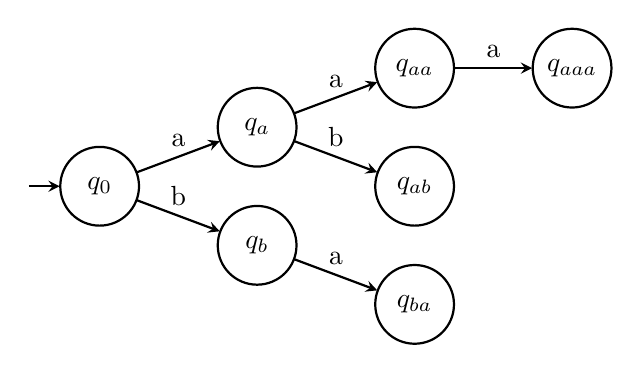
\begin{tikzpicture}[scale=0.5]
\draw[thick] (0,0) circle (1);
\node[circle, minimum size = 10mm] (0) at (0,0) {$q_0$};

\draw[thick] (4,1.5) circle (1);
\node[circle, minimum size = 10mm] (a) at (4,1.5) {$q_{a}$};

\draw[thick] (4,-1.5) circle (1);
\node[circle, minimum size = 10mm] (b) at (4,-1.5) {$q_{b}$};

\draw[thick] (8,3) circle (1);
\node[circle, minimum size = 10mm] (aa) at (8,3) {$q_{aa}$};

\draw[thick] (8,0) circle (1);
\node[circle, minimum size = 10mm] (ab) at (8,0) {$q_{ab}$};

\draw[thick] (8,-3) circle (1);
\node[circle, minimum size = 10mm] (ba) at (8,-3) {$q_{ba}$};

\draw[thick] (12,3) circle (1);
\node[circle, minimum size = 10mm] (aaa) at (12,3) {$q_{aaa}$};

\draw[thick, -{stealth}] (-1.8,0) -- (0);
\draw[thick, -{stealth}] (0) -- (a) node [midway, above] {a};
\draw[thick, -{stealth}] (0) -- (b) node[midway,above]{b};
\draw[thick, -{stealth}] (a) -- (aa) node[midway,above]{a};
\draw[thick, -{stealth}] (a) -- (ab) node[midway,above]{b};
\draw[thick, -{stealth}] (b) -- (ba) node[midway,above]{a};
\draw[thick, -{stealth}] (aa) -- (aaa) node[midway,above]{a};

\end{tikzpicture}
\caption{Prefix tree for the sample $(aa, ab, ba, aaa)$}
\label{fig:pt}
\end{figure}

However, a DFA constructed this way suffers from two main issues making it unsuitable as an interpretable anomaly detector.
On the one hand it overfits the sample $\sample$ and thus poorly generalizes to unseen data.
On the other hand it becomes rather large, hindering interpretability in the sense of Occam's razor.
To overcome these issues we propose an algorithm which not only constructs a DFA fulfilling the given bounds, but also constructs a DFA of minimal size (if one exists).
However, by requiring minimality the problem becomes computationally hard.

More precisely, we can show that the problem whether there exists a DFA
with $n$ states for Problem~\ref{problem:1} is \NP-complete.
We begin by showing that the problem is in \NP, as formalized next.

\begin{theorem}
\label{thm:NP}
    Given a multi-set of words $\sample$, two natural numbers
	$\ell,u \in \mathbb{N}$ with $\ell \leq u \leq \abs{\sample}$,
	and a natural number $n$ (given in unary), a non-deterministic
	Turing machine can compute in polynomial time whether there exists
	a DFA $\dfa$ with $n$ states which accepts at least
	$\ell$ and at most $u$ words from $\sample$ (i.e., the problem
	lies in \NP).
\end{theorem}

\begin{proof} [Proof of Theorem~\ref{thm:NP}]
	Let $\sample,\ell,u,$ and $n$ be given.
    As $n$ is unary, a non-deterministic Turing machine can guess an automaton $\dfa$ with $n$ states.
    The number of accepted words from $\sample$ can then be computed in polynomial time by simulation.
    Finally, checking whether this number is at least $\ell$ and at most $u$ is also possible in polynomial time, showing that the problem lies in \NP.
\end{proof}

Next, we we show \NP-hardness of Problem~\ref{problem:1}, as formalized below.

\begin{theorem}
\label{thm:NP-hard}
	Given a multi-set of words $\sample$, two natural numbers
	$\ell,u \in \mathbb{N}$ with $\ell \leq u \leq \abs{\sample}$,
	and a natural number $n$ (given in unary), the problem of finding
	a DFA $\dfa$ with $n$ states which accepts at least
	$\ell$ and at most $u$ words from $\sample$, is \NP-hard.
\end{theorem}

To proof Theorem~\ref{thm:NP-hard}, we use the \NP-completeness of the following
problem (see \cite{DBLP:books/fm/GareyJ79}).

\begin{problem}\label{problem:NP-Complete}
	Given finite disjoint sets of words $P,N\subseteq\Sigma^*$ and a unary number
	$k\in\mathbb{N}_0$, does there exist a deterministic finite
	automaton $\dfa$ with $k$ states such that $\dfa$
	accepts all words in $P$ and rejects all words in $N$.
\end{problem}

As detailed in the proof below, \NP-hardness (and thus \NP-completeness) of our problem follows
by reduction from Problem \ref{problem:NP-Complete}. This reduction
makes use of the multi-set structure of the samples to encode positive
and negative words from Problem \ref{problem:NP-Complete} in different
multiplicities in the multi-set, which can be distinguished by Problem
\ref{problem:1}.

\begin{proof} [Proof of Theorem~\ref{thm:NP-hard}]
	We show this by a many-one reduction from Problem \ref{problem:NP-Complete}.
	Let finite disjoint sets $P,N\subseteq\Sigma^*$ and a unary number $k\in\mathbb{N}_0$ be given.
	We construct an instance of our problem as follows:
    \begin{itemize}
        \item $n\coloneqq k$;
        \item $\sample(w)\coloneqq\begin{cases}
                                \abs{N}+1&\text{if }w\in P,\\
                                1&\text{if }w\in N,\\
                                0&\text{otherwise,}
        \end{cases}$

		for $w\in\Sigma^*$, i.e., the multi-set contains
		exactly $(\abs{N}+1)$-times all words in $P$ and once all
		words in $N$;
        \item $\ell=u\coloneqq\abs{P}(\abs{N}+1)$.
    \end{itemize}
    This construction can be done in polynomial time.

    Furthermore, if there exists a DFA $\dfa$ with $n$ states solving Problem \ref{problem:1} for $\sample,\ell,$ and $u$ as above, i.e., accepting exactly $\abs{P}(\abs{N}+1)$ words from $\sample$, we have that
    \[
    0\equiv\sum_{w\in P\cup N}\sample(w)\cdot\dfa(w)\equiv\sum_{w\in N}\dfa(w)\pmod{\abs{N}+1}
    \]
    Recall that $\sample(w)$ denotes the number of occurrences of $w$ in $\sample$ and $\dfa(w)$ indicates whether $w$ is accepted by $\dfa$.
	This shows that $\dfa$ rejects all words in $N$, and, thus
    \[
    \abs{P}(\abs{N}+1)=\sum_{w\in P}\sample(w)\cdot\dfa(w)\Rightarrow\abs{P}=\sum_{w\in P}\dfa(w),
    \]
    showing that $\dfa$ accepts all words in $P$ whence $\dfa$ is also a solution to the instance $(P,N,k)$ of Problem \ref{problem:NP-Complete}.

    Similarly, if there exists a DFA $\dfa$ solving the instance $(P,N,k)$ of Problem \ref{problem:NP-Complete}, we have that
    \[
    \sum_{w\in\Sigma^*}\sample(w)\cdot\dfa(w)=(\abs{N}+1)\sum_{w\in P}\dfa(w)=\abs{P}(\abs{N}+1),
    \]
    whence $\dfa$ is also a solution with $n$ states to the instance $(\sample,\ell,u)$ of Problem \ref{problem:1}.

    All in all, this shows the reduction from Problem \ref{problem:NP-Complete}, and thus \NP-hardness of finding a solution of Problem \ref{problem:1} with $n$ states.
\end{proof}


In the first setup, we require the user to provide a lower and an upper bound on the number of anomalies in a given sample.
However this requirement may be to strong.
So in the second setup, which we refer to as \emph{Single-Bound DFA Learning}, we reduce the amount of prior knowledge compared to the first case by alleviating the user’s burden to specify both $\ell$ and $u$.
Instead, we assume to be given a sample $\sample$ and only one parameter, say $\ell$ (the case in which $u$ is given is analogously).
In this case the task is to construct a minimal DFA which accepts at least $\ell$ words from $\sample$.  
In contrast to Problem~\ref{problem:1}, this problem always has a trivial solution since  the DFA which accepts all words in $S$ only has size 1 and fulfills the bound.
However, this DFA underfits the sample $\sample$ and thus does not capture the underlying structure.
To reduce underfitting, we apply a technique commonly applied in automata learning. We construct a DFA of a fixed size which accepts the smallest number $k \geq l$ of words from the sample. 
By providing this size as an additional parameter $n$ the user can regularize the trade-off between avoiding underfitting (larger) and interpretability (smaller).
We propose an algorithm solving this problem which we formally state as:
\begin{problem}[Single-Bound-Learning-Problem]
\label{problem:2}
Given a multi-set of words $\sample = \{w_1, \dots, w_n\}$ and two natural numbers $\ell, n \in \mathbb{N}$ with $\ell \leq \abs{\sample}$, construct a DFA $\dfa$ of size $n$ which accepts the smallest number $k \geq l$ of words from $\sample$.
\end{problem}
This problem is the optimization version of Problem~\ref{problem:1}, thus it is also computationally hard.
In fact, from Problem~\ref{problem:1} being \NP-complete it immediately follows that Problem~\ref{problem:2} lies within the complexity class \NPO (i.e. the class of optimization problems whose decision variant lies in \NP)

\section{Learning via Discrete Optimization}
\label{sec:Learn}
Following a common approach in automata learning we learn a DFA in both setups by reducing the tasks to a set of constraint optimization problems and solve them using state-of-the-art mixed-integer programming solvers (Gurobi in our case~\cite{gurobi}).

\subsection{Two-Bound DFA Learning}
Recall that in the first setup we are given a sample $\mathcal{S}$ and two bounds $\ell, u \in \mathbb{N}$ with $\ell \leq u \leq \abs{\sample}$.
In order to learn a minimal DFA which fulfills these bounds, we apply a technique commonly used in automata learning to ensure minimality. 
The idea is to encode the problem for an automaton of fixed size $n$ such that the encoding has two key properties:
\begin{itemize}
    \item There exists a feasible model if and only if there exists a DFA of size $n$ fulfilling the bounds on the acceptance
    \item This model contains sufficient information to construct such a DFA
\end{itemize}
Starting with an automaton of size one and increasing the size whenever there is no feasible model guarantees to produce the minimal solution.

We now describe the MILP model we use to learn a DFA of size $n$.
Since we just check the existence of a suitable DFA in the first setup, we can choose any constant objective function, e.g. $\mathit{obj} = 1$.
The set of linear inequalities $\Phi_{\sample, \ell, u}^n = \Phi_{\dfa}^n \land \Phi_\mathcal{B}$ consists of two kinds of constraints: 
\emph{automata constrains} $\Phi_{\dfa}^n$, which encode a DFA of size $n$ and the runs on all words from the sample, and \emph{bound constraints} $\Phi_\mathcal{B}$ encoding the bounds on the acceptance.
Throughout these constraints we bound the introduced variables to only take on integer values between (and including) $0$ and $1$, thus simulating boolean variables.

\paragraph{Automata constraints $\Phi_{\dfa}^n$} 
The automata constraints are motivated by the SAT encoding of Biermann and
Feldman~\cite{DBLP:journals/tc/BiermannF72}.
Without loss of generality, the states of the DFA form the set
$Q = \{q_0, \dots, q_{n-1}\}$ where $q_0$ is the initial state.
The alphabet $\Sigma$ of the DFA is the set of all symbols appearing
in the sample $\sample$.
To encode the transitions of the DFA we introduce variables $\delta_{q,a,q'}$ for $q,q' \in Q$ and $a \in \Sigma$.
Intuitively, the variable $\delta_{q,a,q'}$ will be set to 1 if and only if the DFA has a transition from state $q$ to state $q'$ on reading $a$.
Furthermore, we introduce variables $f_q$ for $q \in Q$ which indicate whether a state $q$ is a final state.
To encode the runs of the DFA we start by computing the set of all prefixes in the sample $\mathit{Pref}(\mathcal{S}) = \{ w \mid ww' \in \mathcal{S} \text{ and } w' \in \Sigma^*\}$.
We then introduce a third kind of variable:
$x_{w,q}$ for all $w \in \mathit{Pref}(\mathcal{S})$ and $q \in Q$.
Intuitively, these variables indicate that after reading the prefix $w$ the DFA is in state $q$.\\
%
We now impose constraints on these variables to encode a DFA and its runs. 
Being deterministic there must be precisely one transition for each state $q$ and symbol $a$ which we can model by the following constraint:
\begin{align}
    \sum_{q' \in Q} \delta_{q,a,q'} = 1 \hspace{0.75cm} \forall q \in Q, \forall a \in \Sigma \label{eq:single-transition}
\end{align}
Furthermore, after reading a word $w$ the DFA can only be in one state
\begin{align}
    \sum_{q \in Q} x_{w,q} = 1 \hspace{0.75cm} \forall w \in \mathit{Pref}(S) \label{eq:single-run}
\end{align}
After reading the empty word $\epsilon$ the DFA is in the initial state which we defined to be $q_0$.
This is encoded as:
\begin{align}
    x_{\epsilon,q_0} = 1 \label{eq:initial}
\end{align}
Finally, we encode a run based on the following implication:
\begin{align*}
    x_{w,q} \land \delta_{q,a,q'} \rightarrow x_{wa,q'}
\end{align*}
Intuitively, this implication states that when the DFA is in some state $q$ after reading the word $w$ and there is a transition from $q$ to $q'$ on reading the symbol $a$, then the DFA is in state $q'$ after reading the word $wa$.
As a constraint in MILP we get:
\begin{align}
    x_{w,q} + \delta_{q,a,q'} - 1 \leq x_{wa,q'} \hspace{0.75cm} \notag\\ \forall q, q' \in Q, a \in \Sigma, \forall wa \in \mathit{Pref}(S) \label{eq:run}
\end{align}
We define the automata constraints $\Phi_{\dfa}^n$ to be the conjunction of Equations~\ref{eq:single-transition} to~\ref{eq:run} which concludes the encoding of a DFA of size $n$ and its runs.

\paragraph{Bound constraints $\Phi_\mathcal{B}$}
To impose constraints on the number of accepted words we need to track whether a word $w$ is accepted.
This is the case if and only if after reading $w$ the DFA is in some state $q$ and this state is final.
Intuitively, we could express this case as $x_{w,q} \cdot f_q$, however this is not linear and thus not a valid MILP constraint.
Instead, we exploit the fact that for Boolean variables the multiplication $x_{w,q} \cdot f_q$ is equivalent to the formula $x_{w,q} \land f_q$. 
By introducing fresh variables $\alpha_{w,q}$ for $w \in \sample$ and $q \in Q$ to store the result the later one can be modeled by the following set of constraints:
\begin{align}
    \alpha_{w,q} \geq x_{w,q} + f_q - 1 \hspace{0.75cm} \forall w \in \sample, \forall q \in Q \nonumber\\
    \alpha_{w,q} \leq x_{w,q} \hspace{0.75cm} \forall w \in \sample, \forall q \in Q \label{eq:accepting}\\
    \alpha_{w,q} \leq f_q \hspace{0.75cm}\forall w \in \sample, \forall q \in Q\nonumber
\end{align}
%
Intuitively, the variables $\alpha_{w,q}$ indicate whether a word $w$ is accepted by the DFA (in the state $q$).
Relying on these variables we can encode the bounds on the acceptance as 
\begin{align}
    \sum_{w \in S} \sum_{q \in Q} \alpha_{w,q} \geq \ell\label{eq:lower-bound}\\
    \sum_{w \in S} \sum_{q \in Q} \alpha_{w,q} \leq u\label{eq:upper-bound}
\end{align}
Then the bound constraints $\Phi_\mathcal{B}$ are the conjunction of Equations~\ref{eq:lower-bound} and~\ref{eq:upper-bound}.

After introducing the MILP model we employ it to construct the minimal DFA which fulfills the given bounds on the acceptance.
The idea is to check feasibility of the MILP problem with constant objective function $\mathit{obj} = 1$ and linear inequalities $\Phi_{\sample, \ell, u}^n$ for increasing $n$ until either a solution is found or we reach $n = \abs{\mathit{Pref}(\mathcal{S})} + 2$.
As argued above when proving decidability of problem~\ref{problem:1} the size of the prefix tree is a natural upper bound for the size of the DFA.
Therefore, we can conclude that there exists no DFA fulfilling the given bounds on the sample when we exceed this size.
In the case where a feasible model exists for some size $n$ we construct the corresponding DFA from this model based on the variables $\delta_{q,a,q'}$ and $f_q$.
This procedure is described by Algorithm~\ref{alg:two-bounds}.
\begin{algorithm}
	\caption{Learning with two bounds}\label{alg:two-bounds}
	
	\begin{algorithmic}[1]
		\State \textbf{Input:} Sample $\sample$, Bounds $\ell, u \in \mathbb{N}$
		\State $n\gets 0$
		\Repeat
		\State $n\gets n+1$
		\State Construct $\Phi_{\sample, \ell, u}^n = \Phi_{\dfa}^n \land \Phi_\mathcal{B}$
		\State Set $\mathit{obj} = 1$
		\If{$\mathit{obj},\Phi_{\sample, \ell, u}^n$ has a feasible model (say $m$)}
			\State \Return Construct DFA $\dfa$ using $m$
		\EndIf
		\Until{$n = \abs{\mathit{Pref}(\mathcal{S})} + 2$}
		\State \Return There exists no DFA fulfilling the given bounds
	\end{algorithmic}
\end{algorithm}
%

The correctness of this algorithm is established by the following theorem:

\begin{theorem}
\label{thm:correctness-two-bounds}
Given a sample $\sample$ and two natural numbers $\ell, u \in \mathbb{N}$ with $\ell \leq u \leq \abs{\sample}$, Algorithm~\ref{alg:two-bounds} terminates and outputs a minimal DFA $\dfa_{\sample}$ which accepts at least $\ell$ and at most $u$ words from $\sample$, if such a DFA exists.
\end{theorem}

\begin{proof}	
	We prove Theorem~\ref{thm:correctness-two-bounds} in three steps:
	First, we explain how we construct a DFA from a feasible
	model and proof that this automaton is well-defined and solves
	Problem~\ref{problem:1}.
	Afterwards, we show that a feasible model exists for a size $n$
	if and only if there exists a DFA of that size fulfilling the bounds.
	In the end, we establish termination and show that Algorithm~\ref{alg:two-bounds}
	finds a DFA fulfilling the bounds if such a DFA exists.
	By construction this DFA is minimal.
	
	For now let us assume we found a feasible model for some size $n$.
	We show that the DFA $\dfa=(Q,\Sigma,q_I,\delta,F)$ given by
	\begin{itemize}
		\item $Q=\{q_0,\dots,q_{n-1}\},q_I=q_0;$
		\item $\Sigma$ the symbols present in $\sample$;
		\item $\delta:Q\times\Sigma\rightarrow Q,(q,a)\mapsto q'$
			for $q\in Q,a\in\Sigma,$ and $q'\in Q$ such that
			$\delta_{q,a,q'}$ = 1;
		\item $F\coloneqq\{q\in Q\mid f_q = 1\};$
	\end{itemize}
	is well-defined and solves Problem~\ref{problem:1}.
	First of all, Constraint \ref{eq:single-transition} ensures that the state-transition function $\delta$ is well-defined while $f_q$ simulating Boolean variables further ensures that $F$ is well-defined.
	Next we show that the variables $x_{w,q}$ correspond to the runs of words $w$ from $\sample$ in this well-defined DFA.
	More precisely, we show that $x_{w,q}=1$ if $\dfa$ is in state $q\in Q$ after reading $w\in\mathit{Pref}(\mathcal{S})$ by induction over the prefix length $k=|w|$ (where we w.l.o.g. assume $\sample$ to be non-empty).
	Note that Constraint \ref{eq:single-run} then also ensures the opposite
	direction, i.e., that $\dfa$ is in state $q\in Q$ after reading
	$w\in\mathit{Pref}(\mathcal{S})$ if $x_{w,q}=1$ (as $x_{w,\tilde{q}}=1$
	for the true state $\tilde{q}$ and thus $x_{w,q'}=0\neq1$ for all other
	states $q'\neq\tilde{q}$).
	
	\textit{Base case.} 
	The only prefix of length $k=0$ obviously being the empty word
	$\varepsilon$, Constraint \ref{eq:initial} gives that
	$x_{\varepsilon,q_0}=1$, showing the statement for prefixes of
	length $k=0$.

	\textit{Induction step.}
	Assuming that the statement holds for any prefix of length less or equal to $k$. 
	If no prefix of length $k+1$ exists in $\sample$, the induction is closed and the statement is proven for all prefixes.
	Assume now that $wa\in\mathit{Pref}(\sample)$ is a prefix of length $k+1$.
	Then $w$ is a prefix of length $k$ and thus fulfills for the state
	$q$ reached after reading $w$ in $\dfa$ that $x_{w,q}=1$.
	Writing $q'\coloneqq\delta(q,a)$, Constraint \ref{eq:run} and the
	definition of $\delta$ then give \[x_{w,q} + \delta_{q,a,q'} - 1 = 1 \leq x_{wa,q'}\]
	whence also $x_{wa,q'}=1$ as a Boolean variable.
	As $wa$ was an arbitrary prefix of length $k+1$, this concludes the induction.
	
	While this proofs that the DFA $\dfa$ is well-defined, the bound constraints $\Phi_\mathcal{B}$ ensure that the number of accepted words is above the lower bound $\ell$ and below the upper bound $u$.
	Hence, the DFA $\dfa$ is well-defined and solves Problem~\ref{problem:1}
	
	In a second step, we show that our MILP problem has a feasible
	model for size $n$ if and only if there exists a DFA of size $n$
	that accepts at least $\ell$ and at most $u$ words from $\sample$.

	$(\Rightarrow):$ Given a feasible model for size $n$, we construct a DFA $\dfa$ as explained above.
	As displayed this DFA $\dfa$ is well-defined and fulfills the bounds on the acceptance.

	$(\Leftarrow):$ Given a DFA $\dfa$ of size $n$ which accepts at
	least $\ell$ and at most $u$ words from $\sample$, let the model
	be given by the natural interpretation of the variables:
	\begin{align*} 
		\delta_{q,a,q'} & \coloneqq\begin{cases}
			1&\text{if }\delta(q,a)=q',\\
		    0&\text{otherwise,}
		\end{cases}\\
		f_q & \coloneqq\begin{cases}
			1&\text{if }q\in F,\\
		    0&\text{otherwise,}
		\end{cases}\\
		x_{w,q} & \coloneqq\begin{cases}
			1&\text{if }\dfa\text{ is in state }q\text{ after reading }w,\\
		    0&\text{otherwise,}
		\end{cases} \\
		\alpha_{w,q} & \coloneqq\begin{cases}
			1&\text{if }\dfa\text{ is in state }q\text{ after reading }w\text{ and }q\in F,\\
			0&\text{otherwise,}
		\end{cases}
	\end{align*}
	%
	Being deterministic the DFA $\dfa$ and thus any model constructed this way obviously fulfills Constraints~\ref{eq:single-transition} to~\ref{eq:run}.
	Furthermore, the definition of $\alpha_{w,q}$ ensures that the set of constraints \ref{eq:accepting} is fulfilled and that $\sum_{w\in\sample}\sum_{q\in Q}\alpha_{w,q}=\sum_{w\in\sample}\sum_{q\in F}x_{w,q}$ corresponds to the amount of words in $\sample$ which are accepted by $\dfa$ whence by assumption both Constraint \ref{eq:lower-bound} and Constraint \ref{eq:upper-bound} are fulfilled.
	Hence this model is feasible for our MILP problem for size $n$.

	In order to conclude the proof of Theorem~\ref{thm:correctness-two-bounds} we now show that Algorithm~\ref{alg:two-bounds}
	terminates and finds a DFA fulfilling the bounds if such a DFA exists.
	Termination itself is straight forward.
	The algorithm iterates over increasing sizes until a feasible model is found or $n = \abs{\mathit{Pref}(\mathcal{S})} + 2$ is reached in which case it concludes that no DFA fulfilling the bounds exists.
	Since solving the MILP problem for each $n$ is computable, the algorithm thus always terminates.
	Furthermore, if a feasible model is found, we showed above that the algorithm returns a DFA fulfilling the bounds.
	On the other hand, as explained in the decidability proof of Problem~\ref{problem:1},
	the size of the prefix tree is a natural upper bound for the minimal DFA fulfilling the bounds.
	In the prefix tree, the run on each word $w$ in the sample $\sample$ leads to a unique state $q_w$.
	Therefore, we can check accepting each combination of words from $\sample$ by making the corresponding states a final or non-final state respectively.
	If no such combination fulfills the bounds, we can conclude that no DFA exists which fulfills the bounds.
	Since the prefix tree can have unspecified transitions, we may need one additional state to which we target all these unspecified transitions in order to construct a well-defined DFA.
	Hence, there either exists a DFA of size $n = \abs{\mathit{Pref}(\mathcal{S})} + 1$ or none at all.
	By the equivalence proven above, we thus have that not finding a feasible model until $n = \abs{\mathit{Pref}(\mathcal{S})} + 2$ shows that truly no DFA fulfilling the bounds exists.
	This concludes the proof of termination and correctness and, thus, of Theorem~\ref{thm:correctness-two-bounds}.

	We have shown that Algorithm~\ref{alg:two-bounds} terminates and finds a DFA which fulfills the bounds on the acceptance, if such a DFA exists.
	We displayed that such a DFA of size $n$ exists if and only if our MILP problem for size $n$ has a feasible model.
	Furthermore, we have shown how to construct this DFA given a feasible model.
\end{proof}


Finally, let us investigate the number of constraints in our MILP model.
This number depends on multiple factors:
\begin{itemize}
	\item The size $n$ of the automaton to be constructed
	\item The size of the alphabet $\Sigma$ over which the words in the sample $\sample$ range
	\item The number of unique words in $\sample$
	\item The size of the prefix tree of $\sample$
\end{itemize}
Let $\abs{\Sigma}$ now denote the size of the alphabet and $p =\abs{\mathit{Pref}(\mathcal{S})}$ denote the size of the prefix tree of $\sample$.
Note that the number of unique words in $\sample$ is a lower bound for the size of the prefix tree.
Then, we obtain the following remark.

\begin{remark}
The number of constraints in the MILP problem is in $\mathcal{O}(n^2 \cdot \abs{\Sigma} \cdot p)$.
\end{remark}


\subsection{Single-Bound DFA Learning}
To not clutter this section to much we will only describe the encoding for the case where the lower bound $\ell$ is given. 
The case in which the upper bound is given is analogous.
Recall: If the lower bound $\ell$ is given the task is to construct a DFA of a fixed size $n$ that minimizes acceptance above $\ell$.
Analogously to the first setup we encode the DFA and the runs on all words in the sample using the same set of variables and automata constraints $\Phi_{\dfa}^n$ as above.
Furthermore, we use the same idea to ensure that the number of accepted sequences is larger than the lower bound:
We introduce variables $\alpha_{w,q}$ and add Constraints~\ref{eq:accepting} and~\ref{eq:lower-bound}.
For the remainder of this section let $\Phi_{\ell}$ denote the conjunction of these constraints.
In contrast to Two-Bound-Learning, we not only want to check the existence of a DFA, but also to find the one which minimizes acceptance.
Towards this goal we use the following objective function:
\begin{equation}\label{eq:optimization}
    \mathit{obj} = \min\ \sum_{w \in S} \sum_{q \in Q} \alpha_{w,q}
\end{equation}
which minimizes the number of accepted words from $\sample$
Then we employ this MILP model to construct a DFA of a given size $n$ which minimizes acceptance above the lower bound.
This procedure is described by Algorithm~\ref{alg:lower-bound}.
\begin{algorithm}
	\caption{Learning with a single bound}\label{alg:lower-bound}
	
	\begin{algorithmic}[1]
		\State \textbf{Input:} Sample $\sample$, Bound $\ell \in \mathbb{N}$, Size $n \in \mathbb{N}$
		\State Construct $\Phi_{\sample, \ell}^n = \Phi_{\dfa}^n \land \Phi_{\ell}$
		\State Set $\mathit{obj} = \min\ \sum_{w \in S} \sum_{q \in Q} \alpha_{w,q}$
		\State Compute optimal model minimizing $\mathit{obj}$ with respect to $ \Phi_{\sample, \ell}^n$, say $m$
		
		\State \Return Construct DFA $\dfa$ using $m$
	\end{algorithmic}
\end{algorithm}
%
The correctness of this algorithm is established by the following theorem:
\begin{theorem}
Given a sample $\sample$ and two natural numbers $\ell, n \in \mathbb{N}$ with $\ell \leq \abs{\sample}$, Algorithm~\ref{alg:lower-bound} terminates and outputs a a DFA $\dfa_{\sample}$ of size $n$ which accepts the smallest number $k \geq l$ of words from $\sample$.
\end{theorem}
We omit the proof of this theorem which is similar to the proof of Theorem~\ref{thm:correctness-two-bounds}.

%%% Local Variables:
%%% mode: latex
%%% TeX-master: t
%%% End:
